\documentclass[12pt]{article}
\usepackage{fullpage,enumitem,amsmath,amssymb,graphicx}
\usepackage{listings} % This is a package for including code in your solution.
\usepackage{graphicx} % This is a package for including graphics in your solution.

\title{CS168 Spring Assignment 1}
\author{
	Yueyao Zhu	(yyzhu@stanford.edu) \\
	Yang Du (yd322@stanford.edu)
}

\begin{document}
\maketitle

\section*{Honor Code}

By turning in this assignment, I agree by the Stanford honor code and declare
that all of this is my own work.

\section*{Part 1}

\begin{enumerate}[label=(\alph*)]
 	\item (See code \textbf{simu.py})
 	\item (See \textbf{Figure~\ref{fig:plot}})
	\item 

The strategies of placing balls into bins are analogous to the implementation of hashing with chaining in that:
\begin{enumerate}
	\item Randomly select a bin $\Rightarrow{}$ Perform a universal hashing function
	\item Check the number of balls in a bin $\Rightarrow{}$ Get the length of the linked list of the hash table bucket, i.e. the number of chaining objects in the bucket
	\item Place a ball into a bin $\Rightarrow{}$ Add the object to the linked list of the hash table bucket
\end{enumerate}

Therefore, strategy (a) suggests implementing chaining hashing with one hash function $H$, and storing the object $o$ into the bucket (linked list) $\#H(o)$. Strategy (b), (c) suggest using multiple hash functions $H_1, H_2, ..., H_n$, and storing the object into the one (linked list) with the lowest occupancy (list length) among buckets $\#H_1(o), \#H_2(o), .. \#H_n(o)$, where ties are broken with a random selection. $n=2$ in strategy (b) and $n=3$ in strategy (c).

Strategy (d) suggests having two sets of buckets $B_1$, $B_2$, and use hash functions $H_1:O\rightarrow{}B_1$, $H_2:O\rightarrow{}B_2$ to choose one bucket from each sets. The object is put into the one with fewer objects (shorter linked list) and ties are broken by choosing the one from $B_1$.

% The trade-offs exist since a more complex insertion algorithms (using more hash functions and choosing a bucket wisely to lower collision thus the length of each bucket) will increase the insertion time, but lower the number of items in a hash bucket thus decreasing the worst-case search time, and vise versa.

% Strategy (a) is the most common one used. It is most possible for strategy (a) among all that there will be a collision so that a hash table bucket will contain a large amount of objects and longer time to access an object which requires a linear search on the whole chain of the bucket. Strategy (b) and (c) increases the complexity of the insertion algorithm (more hash function calculations and bucket length comparisons) and the insertion time, but they will lower the chances of the collision and thus less time is consumed to access an object.

The first strategy is the most common one we used. It is very possible that there will be a collision so that a bucket will contain a large amount of objects so that the time to access an objects requires a linear search on the whole chaining in the bucket.

The second strategy require one more hash function, so that for each of the new objects, it will cost the program to calculate one more times. But it will cause less collision.
The third strategy requires three hash functions so that three calculations are needed, but less collisions.
The fourth strategy either requires double space, or make each hash bucket received double elements. If we use double space, then the collision will decrease, but if we keep the space be the same, and use two hash function separately, then each bucket will have a higher chance to be hashed in.
\end{enumerate}

\begin{figure}[h]
	\centering
	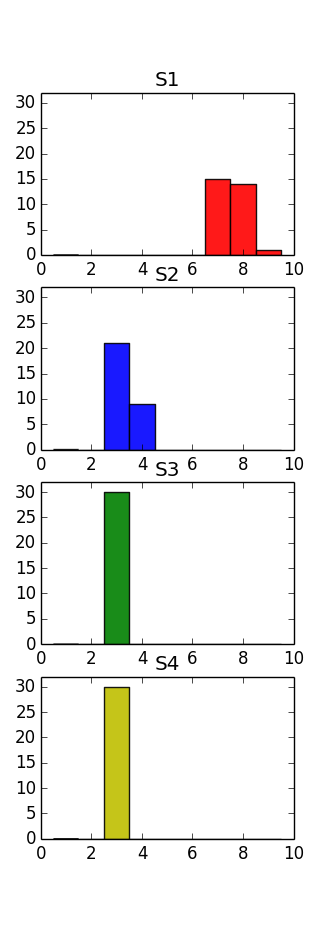
\includegraphics[width=0.4\textwidth]{figure_1.png}
	\caption{Histogram for $X$}
	\label{fig:plot}
\end{figure}

\end{document}